\documentclass[a4paper]{article}
\usepackage{array}
\usepackage{datetime}
\usepackage{color}
\usepackage{url}
\usepackage{hyperref}
\usepackage{graphicx}
\usepackage{caption}
\usepackage{subcaption}
\usepackage{listings}
\usepackage{xcolor}
\usepackage[T2A]{fontenc}
\usepackage[utf8]{inputenc}
\usepackage{amssymb}
\usepackage[english,serbianc]{babel}

\hypersetup{
    colorlinks,
    linkcolor=blue,
    urlcolor=blue
}

%%%%%%%%%% JSON DARK MAGIC %%%%%%%%%%
\newcommand\JSONnumbervaluestyle{\color{blue}}
\newcommand\JSONstringvaluestyle{\color{red}}

% switch used as state variable
\newif\ifcolonfoundonthisline

\makeatletter

\lstdefinestyle{json}
{
  showstringspaces    = false,
  keywords            = {false,true},
  alsoletter          = 0123456789.,
  morestring          = [s]{"}{"},
  stringstyle         = \ifcolonfoundonthisline\JSONstringvaluestyle\fi,
  MoreSelectCharTable =%
    \lst@DefSaveDef{`:}\colon@json{\processColon@json},
  basicstyle          = \ttfamily,
  keywordstyle        = \ttfamily\bfseries,
}

% flip the switch if a colon is found in Pmode
\newcommand\processColon@json{%
  \colon@json%
  \ifnum\lst@mode=\lst@Pmode%
    \global\colonfoundonthislinetrue%
  \fi
}

\lst@AddToHook{Output}{%
  \ifcolonfoundonthisline%
    \ifnum\lst@mode=\lst@Pmode%
      \def\lst@thestyle{\JSONnumbervaluestyle}%
    \fi
  \fi
  %override by keyword style if a keyword is detected!
  \lsthk@DetectKeywords% 
}

% reset the switch at the end of line
\lst@AddToHook{EOL}%
  {\global\colonfoundonthislinefalse}

\makeatother
%%%%%%%%%%%%%%%%%%%%%%%%%%%%%%%%%%%%%

\begin{document}

\title{
Систем за лабелирање "Каникс"\\
\small{
	Семинарски рад у оквиру курсева\\
	програмирање Веб\\
	Функционално програмирање\\
	Математички Факултет
	}
}

\author{Урош Стегић 447/2016\\ urosstegic@gmx.com}
\date{\today}
\maketitle

\tableofcontents
\clearpage

\section{Опис проjекта}
Потребно jе израдити систем за контролисано лабелирање рукописа.
Под лабелирањем рукописа се подразумева писање jедног задатог карак-
тера тj. његово цртање на екрану. Како се не би нарушавала аутентичност
руком писаних симбола, неопходно jе подржати технологиjу коjа омогућава
цртање слободном руком па ће према томе Каникс подржавати искључиво
таблет уређаjе и паметне телефоне са екраном осетљивим на додир. По-
дршка за стоне и преносиве рачунаре неће постоjати. Зарад праћења ра-
зличитих рукописа, потребно jе омогућити корисницима креирање личног
налога, верификациjу имеjл адресе и логовање на систем. Поред овога, за
праћење разних статистичких података, извоз означених карактера у од-
говараjућем формату, контролу карактера коjе jе могуће означавати и jош
много других ствари, потребно jе развити администраторски панел у коме
ће администратор система моћи олакшано да управља садржаjем аплика-
циjе и у коме ће имати увид у количину и разноврсност лабелираног мате-
риjала. Како би се процес лабелирања учинио забавниjим уводи се концепт
поена и достигнућа. Након сваког нацртаног карактера корисник осваjа
известан броj поена и тим поенима се пење уз лествицу достигнућа. Ани-
мираност овог процеса има за циљ да учини означавање рукописа jош мање
мукотрпним послом. Након довољно прикупљених података (коришћењем
неких основних техника машинског учења) систем ће моћи да самостално
одбацуjе слике коjе се драстично разликуjу од онога што се очекуjе од кори-
сника да нацрта. Означене карактере jе потребно чувати без непотребних
информациjа у векторском формату. Сваки потез коjи корисник нацрта ће
бити репрезентован минималним скупом тачака коjе формираjу отворену
криву. Jедан караткер jе представљен скупом од jедне или више кривих.
Даљи рад на овом алату може бити адаптациjа у игру коjа се може кори-
стити у едукативне сврхе за децу предшколског узраста помоћу коjе би она
учила да пишу, али то излази из оквира овог семинарског рада.

\section{Техничка спецификациjа}
Алат ће бити развиjен као Веб апликациjа фокусирана на кориснике мо-
билних телефона и таблета. На серверскоj страни ће бити развиjен РЕСТ
АПИ, док ће клиjентска страна бити имплементирана као jеднострана апли-
кациjа (\textit{eng. Single page application, SPA}).\\

\subsection{Серверска страна:}
\begin{itemize}
	\item Хаскел;
	\item Jесод радни оквир (\textit{eng. Yesod});
	\item Персистант (\textit{eng. Persistant}) - ОРМ слоj;
	\item МонгоДБ нерелациона база података.
\end{itemize}

\subsection{Клиjентска страна:}
\begin{itemize}
	\item ХТМЛ5 / ЦСС3;
	\item Твитер Бутстреп ЦСС радни оквир;
	\item Реакт радни оквир;
	\item Канвас АПИ.
\end{itemize}


\section{План рада}
Начелно, план израде проjекта jе подељен у три категориjе: фаза проjек-
товања, фаза имплементациjе и фаза додатних захтева, али се током израде
могу очекивати извесна одступања. Називи ових фаза нису стриктни ни у
ком погледу и за циљ имаjу да пруже глобалну слику делова развоjа. Та-
кође, делови тих фаза неће бити наведени у хронолошком редоследу. Фаза
додатних захтева представља опциона своjства система и њихова израда
зависи од времена коjу одузме основни део.

\subsection{Фаза проjектовања}
\begin{itemize}
	\item Скица корисничког интерфеjса;
	\item Дизаjнирање РЕСТ АПИ-jа;
	\item Проjектовање базе.
\end{itemize}

\subsection{Фаза имплементациjе}
\begin{itemize}
\item Серверски део апликациjе\\
Првенствено ће бити развиjен РЕСТ АПИ према готовом дизаjну.
Нема потребе сада детаљно описивати делове АПИ-jа и целокупног
система jер ће они бити описани у наставку.

\item Графички интерфеjс\\
Према скици из претходне фазе израђуjе се кориснички интерфеjс.
Наравно, неће бити израђен комплетан интерфеjс jер он зависи од
касниjих делова имплементациjе, али костур и статични садржаj ће
бити постављени у овоj фази.

\item Кориснички систем\\
Код корисничког система jе у основи неопходно развити могућност
креирања налога и механизам приjављивања на систем. Поред тога,
корисници ће имати могућност да измене корисничко име, лозинку и
фотографиjу профила, као и да прегледаjу статистику своjих ознака.
Уклањање налога ниjе могуће.

\item Администраторски панел\\
Основни администраторски панел мора омогућити администратору
преглед информациjа о означеним (лабелираним) карактерима (укупно
и по кориснику), приказ узорка тих ознака и могућност одбацивања
ознаке уз одговараjућу поруку.

\item Навигациjа кроз апликациjу\\
Како ће садржаj бити подељен у различите категориjе (мала слова,
велика слова, броjеви, интерпункциjски знаци итд.) потребно jе до-
хватити одговараjуће ресурсе са сервера и оспособити навигациjу кроз
ове категориjе и одабир карактера коjи се црта. Такође за сваку кате-
гориjу и сваки карактер jе потребно приказати основне информациjе о
томе колико карактера jе из дате категориjе нацртано, односо колико
пута jе дати карактер нацртан.

\item Цртање карактера\\
Кључан део апликациjе представља цртање одабраног карактера. По-
требно jе омогућити цртање карактера, слање цртежа на сервер и ди-
ректну навигациjу ка претходном и следећем карактеру како би се
олакшало кретање кроз апликациjу.
\end{itemize}

\subsection{Фаза додатних захтева}
Међу додатне захтеве спадаjу неке напредниjе функционалности као
што су: алгоритам К наjближих суседа коjи за циљ има аутоматско од-
бацивање (сугерисање администратору) сумњивих фотографиjа. Такође
систем бодова и награда jе опциони. Омогућавање ове функционалности
изискуjе више креативног рада, осмишљавања награда, цртање или прона-
лажење иконица него демонстрациjе знања па се из тог разлога сврстава у
ову категориjу.

\section{Опис визуелног интефеjса}
Како бисмо се лакше упознали са апликациjом наjбоље jе почети од
графичког корисничког интерфеjса. У овом одељку ће бити описани сви
екрани апликациjе и биће приказане скице тих екрана.

\subsection{Почетна страна}
Почетном екрану се приступа инициjалним покретањем апликациjе. Уко-
лико корисник ниjе приjављен на систем, на почетноj страници се налазе
само линкови за приjављивање и за регистрациjу и сви остали де-
лови апликациjе му нису доступни. Улогован корисник не види оваj екран
и њему се приказуjу статусна линиjа са процентом завршености следећи
линкови:
\begin{itemize}
	\item \hyperref[personal]{лична страна};
	\item \hyperref[categories]{категориjе};
	\item \hyperref[help]{помоћ};
	\item одjава;
\end{itemize}

\begin{figure}
\centering
\begin{subfigure}{.5\textwidth}
  \centering
  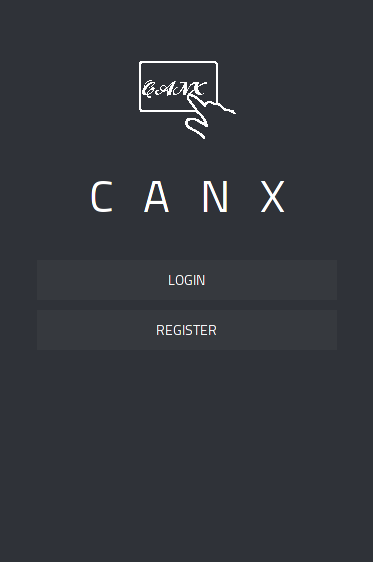
\includegraphics[width=.9\linewidth]{home_noauth}
  \caption{Посетиоци}
  \label{fig:sub1}
\end{subfigure}%
\begin{subfigure}{.5\textwidth}
  \centering
  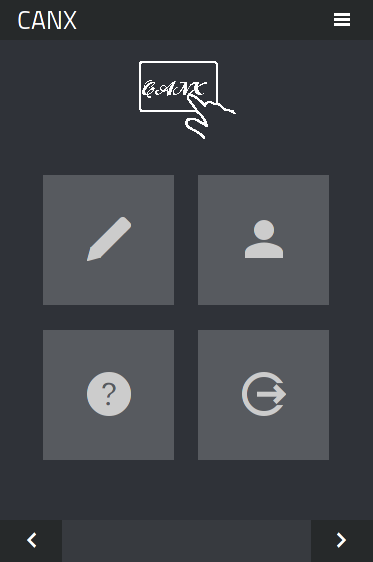
\includegraphics[width=.9\linewidth]{home_auth}
  \caption{Пријављени корисници}
  \label{fig:sub2}
\end{subfigure}
\caption{Почетни екран}
\label{fig:test}
\end{figure}

\subsection{Лична страна}
\label{personal}
На овоj страни корисник може подесити/изменити своjе корисничко име,
меjл адресу, аватар и лозинку.

\subsection{Категориjе}
\label{categories}
Са ове странице корисник може да одабере коjе категориjу карактера
коjе жели да исцртава. Основна верзиjа апликациjе ће подржавати следеће
категориjе:
\begin{itemize}
	\item велика слова;
	\item мала слова;
	\item цифре;
	\item математичке симболе;
\end{itemize}
Одабиром категориjе се отвара екран са \hyperref[character]{избором карактера}. На пример,
ако jе корисник изабрао категориjу "велика слова", отвориће се екран на
коме ће имати избор великих слова за цртање. У оквиру сваке категориjе
ће бити приказан проценат попуњености те категориjе (однос нацртаних
карактера те категориjе и жељеног броjа карактера).

\subsection{Карактер}
\label{character}
На екрану за избор карактера за цртање се налазе дугмићи са листом
карактера изабране категориjе. Одабиром карактера се отвара \hyperref[canvas]{платно} за
цртање тог карактера. У оквиру сваког карактера ће се налазити броj
облика 4/10 коjи представља броj нацртаних карактера и броj жељених
карактера. У случаjу да jе корисник нацртао потребан броj карактера неће
се налазити броj на том месту већ симбол "\checkmark" и корисник више неће бити у
могућности да црта таj карактер. Како корисник не би морао да се враћа на
претходни екран зарад избора друге категориjе, кретање кроз категориjе jе
могуће директно са овог екрана, помоћу дугмића "<" и ">" коjи се налазе
у футеру.

\begin{figure}
\centering
\begin{subfigure}{.5\textwidth}
  \centering
  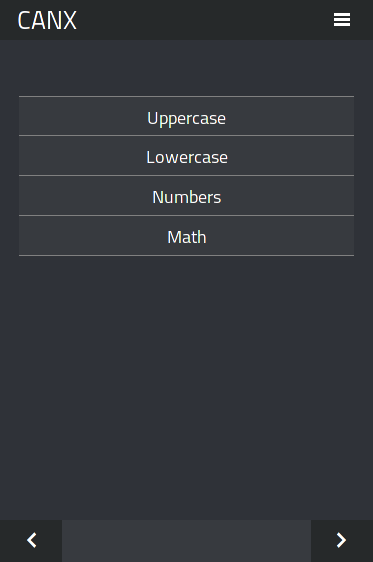
\includegraphics[width=.9\linewidth]{categories}
  \caption{Избор категорије}
  \label{fig:sub1}
\end{subfigure}%
\begin{subfigure}{.5\textwidth}
  \centering
  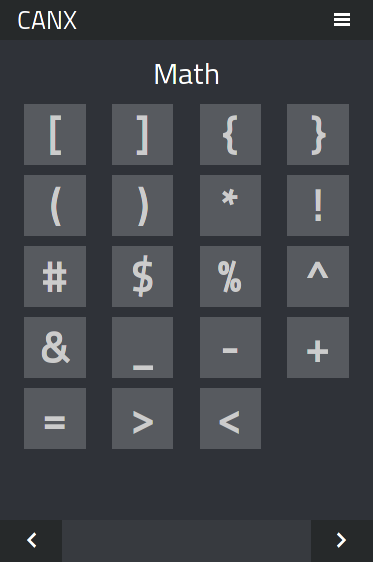
\includegraphics[width=.9\linewidth]{letters}
  \caption{Избор карактера}
  \label{fig:sub2}
\end{subfigure}
\caption{Навигација кроз карактере}
\label{fig:test}
\end{figure}

\subsection{Платно}
\label{canvas}
Када смо одабрали карактер коjи желимо да цртамо, на овом екрану га
можемо нацртати. Када нацртамо карактер и задовољни смо њиме, можемо
га послати на обраду кликом на дугме за слање (дугме са ознаком "\checkmark").
Платно можемо очистити дугметом са иконицом корпе. Дугмићима "<" и
">" се можемо кретати кроз карактере директно са овог екрана. Приликом
слања се врши примитивна провера садржаjа, тj. одбацуjу се нацрти коjи
не садрже ни jедан потез или коjи садрже превише потеза. Репрезентациjа
нацртане слике и начин слања ће бити описани у одељку са описом РЕСТ
АПИ-jа.

\subsection{Помоћ}
\label{help}
Страница "Помоћ" је статичка страна у којој ће бити описана употреба апликације. Поред тога ће садржати често постављана питања, контакт информације аутора и томе сличне податке.

\subsection{Oстало}
Поред главних графичких елемената тј. страница апликације имамо и помоћне помоћне компоненте.
\begin{itemize}
\item брза навигација\\
Када се корисник одабере категорију карактера које жели да црта, како зарад избора друге категорије не би морао да се враћа на претходни екран, кретање по категоријама је олакшано. Стрелице из футера апликације служе за брз прелазак на претходну/следећу категорију. Аналогно за кретање кроз карактере.
\item навигациони панел\\
Претходна навигација се односила на кретање кроз категорије и карактера. Главна навикација коју имамо на почетном екрану је доступна и кроз хамбургер мени који се налази у заглављу сваке странице. Притиском на то дугме се отвара падајућа листа која садржи опције идентичне онима које се налазе на почетној страни.
\item модални прозор\\
Одређене корисничке акције попут одјављивања са система и слања нацртаног карактера захтевају додатну потврду. Пре извршавања акције се приказује модални прозор који садржи одговарајућу поруку и два дугмета: дугме за потврду и дугме за поништавање акције.
\end{itemize}
\begin{figure}
\centering
\begin{subfigure}{.5\textwidth}
  \centering
  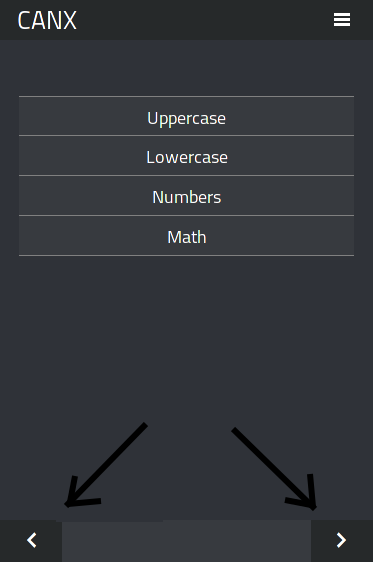
\includegraphics[width=.9\linewidth]{fast_nav}
  \caption{Брза навигација}
  \label{fig:sub1}
\end{subfigure}%
\begin{subfigure}{.5\textwidth}
  \centering
  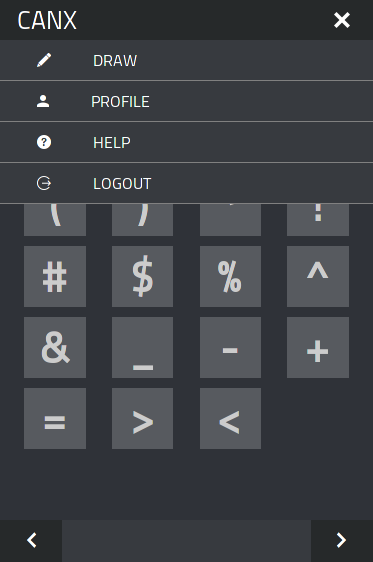
\includegraphics[width=.9\linewidth]{hamburger}
  \caption{Навигациони панел}
  \label{fig:sub2}
\end{subfigure}
\caption{Помоћне графичке компоненте}
\label{fig:test}
\end{figure}

\section{Серверска страна}
Три главне компоненте серверске стране су дефинисање ресурса тј. РЕСТ интерфејса, складиштење података кроз СУБП и аутентификација корисника и заштита ресурса.

\subsection{РЕСТ Интерфејс}
Пре описивања свих ресурса унутар система, битно је нагласити да се овде појам ресурс односи на објекте који ће бити складиштени у бази података тј. то ће бити објекти који се могу разматрати само у контексту података. Дакле, не обраћамо пажњу на све ресурсе који се преносе ка клијенту као што су јаваскрипт датотеке, датотеке са стиловима, фотографије и слично иако је њихова улога значајна у систему. Сви ресурси које препознајемо  подржавају све ПЧМБ операције и они су у складу са класичном дефиницијом РЕСТ интерфејса. Сви ресурси РЕСТ АПИ-ја су префиксовани са \lstinline[basicstyle=\ttfamily\color{black}]|/api|,  мада ће у опису интерфејса бити експлицитно наведени.

\begin{itemize}
\item \lstinline[basicstyle=\ttfamily\color{black}]|/api/users/123456| - корисник система са идентификатором 123456
\begin{lstlisting}[style=json]
{
    "uid": 123456,
    "name": "John Doe",
    "email": "john.doe@gmail.com",
    "pass": "5f4dcc3b5aa765d61d8327deb882cf99",
    "avatar": "/avatars/john_doe.png",
    "characters": [
    {
        "name": "a",
        "category": "lowercase",
        "drawing": "<svg>..."
    },
    {
        "name": "a",
        "category": "lowercase",
        "drawing": "<svg>..."
    }
    ]
}
\end{lstlisting}

\item \lstinline[basicstyle=\ttfamily\color{black}]|/api/categories/lowercase| - категорија карактера са идентификатором "lowercase"
\begin{lstlisting}[style=json]
{
    "cid": "lowercase",
    "name": "Lowercase Letters",
    "characters": ["a", "b", "c", ..., "z"]
}
\end{lstlisting}
\clearpage
\item \lstinline[basicstyle=\ttfamily\color{black}]|/api/characters/plus| - опис карактера са идентификатором "plus"
\begin{lstlisting}[style=json]
{
    "chid": "plus",
    "category": "math",
    "symbol": "+"
}
\end{lstlisting}

\end{itemize}
Поред основних интерфејса ка ресурсима, у складу са РЕСТ архитектуром постоје интерфејси ка колекцијама ресурса. Ови интерфејси служе искључиво за читање садржаја и можемо им приступити само \textit{GET} методом. То су интерфејси:
\begin{itemize}
\item \lstinline[basicstyle=\ttfamily\color{black}]|/api/users|
\item \lstinline[basicstyle=\ttfamily\color{black}]|/api/categories|
\item \lstinline[basicstyle=\ttfamily\color{black}]|/api/characters|
\end{itemize}

\subsection{Безбедност}
Како приступ ресурсима имају искључиво корисници који су пријављени на систем, потребно је обезбедити слој заштите тих ресурса. За ове потребе је употребљен механизам пријављивања \textit{OAuth 2.0} који је прикључен пакетом \textit{yesod-auth-oauth2}.
TODO: опис интерфејса за логовање и заштиту ресурса.

\subsection{База података}
TODO: опис базе, бакета итд...

\end{document}
